\chapter{Phonons, Rotons and the Dispersion Relation}\label{ch05}
% generated by ch05_numbers.py -- do not edit
\expandafter\def\csname cfive@tableRows\endcsname{1\,727}
\expandafter\def\csname cfive@nErrRows\endcsname{34}
\expandafter\def\csname cfive@kmax\endcsname{3.6}
\expandafter\def\csname cfive@c\endcsname{238.3}
\expandafter\def\csname cfive@kDense\endcsname{3.44}
\expandafter\def\csname cfive@maxonKshort\endcsname{1.1}
\expandafter\def\csname cfive@maxonE\endcsname{1.19}
\expandafter\def\csname cfive@rotonE\endcsname{0.741}
\expandafter\def\csname cfive@rotonGapK\endcsname{8.60}
\expandafter\def\csname cfive@rotonKshort\endcsname{1.92}
\expandafter\def\csname cfive@rotonMass\endcsname{0.141}
\expandafter\def\csname cfive@landauV\endcsname{57.9}
\expandafter\def\csname cfive@landauK\endcsname{1.97}
\expandafter\def\csname cfive@landauOverC\endcsname{0.243}
\expandafter\def\csname cfive@landauQuad\endcsname{57.9}
\expandafter\def\csname cfive@landauQuadPct\endcsname{0.01}
\expandafter\def\csname cfive@phaseMaxPct\endcsname{5.4}
\expandafter\def\csname cfive@vphLow\endcsname{238.5}
\expandafter\def\csname cfive@phaseMaxPctAlt\endcsname{5.3}
\expandafter\def\csname cfive@phaseMaxK\endcsname{0.35}
\expandafter\def\csname cfive@kGroup\endcsname{0.404}
\expandafter\def\csname cfive@kSym\endcsname{0.455}
\expandafter\def\csname cfive@kPhase\endcsname{0.566}
\expandafter\def\csname cfive@kSymTable\endcsname{0.453}
\expandafter\def\csname cfive@shiftG\endcsname{0.002}
\expandafter\def\csname cfive@shiftP\endcsname{0.005}
\expandafter\def\csname cfive@symMax\endcsname{14.5}
\expandafter\def\csname cfive@symMaxK\endcsname{0.31}
\expandafter\def\csname cfive@seriesDevMax\endcsname{2.2}
\expandafter\def\csname cfive@kstar\endcsname{3.00}
\expandafter\def\csname cfive@alphaBog\endcsname{0.055}
\expandafter\def\csname cfive@alphaRatio\endcsname{28}
\expandafter\def\csname cfive@h2m4\endcsname{0.522}
\expandafter\def\csname cfive@resFWHM\endcsname{0.07}
\expandafter\def\csname cfive@nPixBin\endcsname{70}
\expandafter\def\csname cfive@err03ueV\endcsname{1.0}
\expandafter\def\csname cfive@bend03ueV\endcsname{23}
\expandafter\def\csname cfive@rotonYat\endcsname{0.25}
\expandafter\def\csname cfive@vgMax\endcsname{1.08}
\expandafter\def\csname cfive@vgMaxPct\endcsname{8.5}
\expandafter\def\csname cfive@vgMaxK\endcsname{0.27}
\expandafter\def\csname cfive@vgCrossK\endcsname{0.40}
\expandafter\def\csname cfive@vgZeroK\endcsname{1.10}
\expandafter\def\csname cfive@vgMin\endcsname{-0.57}
\expandafter\def\csname cfive@vgMinK\endcsname{1.63}
\expandafter\def\csname cfive@exLandau\endcsname{58.0}
\expandafter\def\csname cfive@mfMaxK\endcsname{0.56}
\expandafter\def\csname cfive@mfMaxW\endcsname{0.350}
\expandafter\def\csname cfive@mfMinK\endcsname{0.84}
\expandafter\def\csname cfive@mfMinW\endcsname{0.304}
\expandafter\def\csname cfive@mfLandau\endcsname{0.349}
\expandafter\def\csname cfive@mfLandauK\endcsname{0.90}
\expandafter\def\csname cfive@pLandau0\endcsname{57.9}
\expandafter\def\csname cfive@pLandau24\endcsname{46.1}
\expandafter\def\csname cfive@pRatio0\endcsname{0.243}
\expandafter\def\csname cfive@pRatio24\endcsname{0.127}
\expandafter\def\csname cfive@pC24\endcsname{362}
\expandafter\def\csname cfive@pCrise\endcsname{52}
\expandafter\def\csname cfive@pRoton24\endcsname{0.626}
\expandafter\def\csname cfive@pKR24\endcsname{2.05}
\expandafter\def\csname cfive@pP24\endcsname{24.08}
\expandafter\def\csname cfive@pKmaxRange\endcsname{2.2}
\expandafter\def\csname cfive@nModesMain\endcsname{3208}
\expandafter\def\csname cfive@nmodesRetained\endcsname{3209}
\expandafter\def\csname cfive@nModesG2\endcsname{796}
\expandafter\def\csname cfive@Tmain\endcsname{300}
\expandafter\def\csname cfive@nGolden\endcsname{28}
\expandafter\def\csname cfive@secRun\endcsname{65}
\expandafter\def\csname cfive@secFit\endcsname{12}
\expandafter\def\csname cfive@medMain\endcsname{0.60}
\expandafter\def\csname cfive@p99Main\endcsname{8.5}
\expandafter\def\csname cfive@maxMain\endcsname{26}
\expandafter\def\csname cfive@medG2\endcsname{0.42}
\expandafter\def\csname cfive@medSplit\endcsname{1.2}
\expandafter\def\csname cfive@medLowK\endcsname{3.8}
\expandafter\def\csname cfive@medHighK\endcsname{0.33}
\expandafter\def\csname cfive@nBand\endcsname{3128}
\expandafter\def\csname cfive@zMin\endcsname{-0.976}
\expandafter\def\csname cfive@zMax\endcsname{-0.488}
\expandafter\def\csname cfive@zDev\endcsname{0.009}
\expandafter\def\csname cfive@ladA\endcsname{\ensuremath{3.6\times10^{-7}}}
\expandafter\def\csname cfive@ladB\endcsname{\ensuremath{2.3\times10^{-8}}}
\expandafter\def\csname cfive@ladC\endcsname{\ensuremath{1.4\times10^{-9}}}
\expandafter\def\csname cfive@ratioA\endcsname{15.6}
\expandafter\def\csname cfive@ratioB\endcsname{16.8}
\expandafter\def\csname cfive@ladVsFit\endcsname{26}
\expandafter\def\csname cfive@collapseA\endcsname{\ensuremath{2.6\times10^{-5}}}
\expandafter\def\csname cfive@collapseB\endcsname{\ensuremath{1.7\times10^{-5}}}
\expandafter\def\csname cfive@labK\endcsname{1.571}
\expandafter\def\csname cfive@labOmega\endcsname{1.9974}
\expandafter\def\csname cfive@labPeakA\endcsname{-2.9975}
\expandafter\def\csname cfive@labPeakB\endcsname{0.9974}
\expandafter\def\csname cfive@labExpA\endcsname{-2.9974}
\expandafter\def\csname cfive@labExpB\endcsname{0.9974}
\expandafter\def\csname cfive@ampK1\endcsname{0.393}
\expandafter\def\csname cfive@ampK2\endcsname{1.571}
\expandafter\def\csname cfive@ampS1\endcsname{\ensuremath{-2.7\times10^{-5}}}
\expandafter\def\csname cfive@ampS2\endcsname{\ensuremath{-2.6\times10^{-3}}}
\expandafter\def\csname cfive@ampS3\endcsname{\ensuremath{-2.2\times10^{-2}}}
\expandafter\def\csname cfive@ampS3pct\endcsname{2.2}
\expandafter\def\csname cfive@ampR1\endcsname{0.19}
\expandafter\def\csname cfive@unkMain\endcsname{6\,418}
\expandafter\def\csname cfive@relSys\endcsname{2.1\times10^{-3}}
\expandafter\def\csname cfive@phaseMaxRatio\endcsname{1.054}
\expandafter\def\csname cfive@vgKcut\endcsname{3.19}
\expandafter\def\csname cfive@ringRmin\endcsname{11}
\expandafter\def\csname cfive@ringRmax\endcsname{28}
\expandafter\def\csname cfive@ringKmin\endcsname{0.8}
\expandafter\def\csname cfive@ringKmax\endcsname{3.1}
\expandafter\def\csname cfive@ringMed\endcsname{3.4}
\expandafter\def\csname cfive@ringMax\endcsname{13}
\expandafter\def\csname cfive@cvN\endcsname{16}
\expandafter\def\csname cfive@cvModes\endcsname{49}
\expandafter\def\csname cfive@cvUnknowns\endcsname{98}
\expandafter\def\csname cfive@cvT\endcsname{20}
\expandafter\def\csname cfive@cvRustSec\endcsname{0.3}
\expandafter\def\csname cfive@cvRk4Dt\endcsname{\ensuremath{5.3\times10^{-7}}}
\expandafter\def\csname cfive@cvEta\endcsname{10^{-4}}
\expandafter\def\csname cfive@cvErr4\endcsname{\ensuremath{7.8\times10^{-4}}}
\expandafter\def\csname cfive@cvErr6\endcsname{\ensuremath{2.7\times10^{-5}}}
\expandafter\def\csname cfive@cvErr8\endcsname{\ensuremath{2.7\times10^{-7}}}
\expandafter\def\csname cfive@cvErr10\endcsname{\ensuremath{3.3\times10^{-9}}}
\expandafter\def\csname cfive@cvBogMax\endcsname{\ensuremath{3.3\times10^{-4}}}
\expandafter\def\csname cfive@cvPerMin\endcsname{1.3}
\expandafter\def\csname cfive@cvPerMax\endcsname{6.4}
\expandafter\def\csname cfive@cvFineErr\endcsname{\ensuremath{2.1\times10^{-9}}}
\expandafter\def\csname cfive@cvBestTol\endcsname{\ensuremath{10^{-10}}}
\expandafter\def\csname cfive@cvBestErr\endcsname{\ensuremath{3.3\times10^{-9}}}
\expandafter\def\csname cfive@cvBestTraj\endcsname{\ensuremath{8.0\times10^{-7}}}
\expandafter\def\csname cfive@cvScale8\endcsname{365}
\expandafter\def\csname cfive@cvScale16\endcsname{710}
\expandafter\def\csname cfive@cvScale32\endcsname{2\,291}
\expandafter\def\csname cfive@cvScaleSec8\endcsname{0.2}
\expandafter\def\csname cfive@cvScaleSec16\endcsname{0.5}
\expandafter\def\csname cfive@cvScaleSec32\endcsname{9.4}
\expandafter\def\csname cfive@cvScaleUnk8\endcsname{26}
\expandafter\def\csname cfive@cvScaleUnk16\endcsname{98}
\expandafter\def\csname cfive@cvScaleUnk32\endcsname{394}
\expandafter\def\csname cfive@unkRatio\endcsname{16}
\expandafter\def\csname cfive@cvSmallN\endcsname{8}
\expandafter\def\csname cfive@cvGrowOldA\endcsname{7}
\expandafter\def\csname cfive@cvGrowOldB\endcsname{9}
\expandafter\def\csname cfive@cvOldFallA\endcsname{11}
\expandafter\def\csname cfive@cvOldFallB\endcsname{10}
\expandafter\def\csname cfive@cvOldDate\endcsname{26 September 2026}
\expandafter\def\csname cfive@cvRatio4\endcsname{2}
\expandafter\def\csname cfive@cvRatio6\endcsname{14}
\expandafter\def\csname cfive@cvOldErr6\endcsname{\ensuremath{1.7\times10^{-3}}}
\expandafter\def\csname cfive@cvNewErr6\endcsname{\ensuremath{1.7\times10^{-5}}}
\expandafter\def\csname cfive@cvRatio8\endcsname{92}
\expandafter\def\csname cfive@nAxiomLines\endcsname{15}

\providecommand{\cfiveV}[1]{\ifcsname cfive@#1\endcsname\csname cfive@#1\endcsname\else\textbf{??#1??}\PackageWarning{ch05}{undefined number key #1}\fi}
\providecommand{\cfiveAng}{\text{\AA}}
\providecommand{\cfivepath}[1]{{\urlstyle{tt}\path{#1}}}

%% ====================================================================================================================
\section{A curve read off a spectrometer}\label{ch05:sec-curve}

Keep a cell of liquid helium below a tenth of a kelvin, send cold neutrons of known energy through it, and note which of them come out having left energy behind.
A neutron that has created exactly one excitation of the liquid --- one phonon, one roton --- is found to have lost a definite energy $\varepsilon$ while its direction changed by an amount that fixes a definite momentum transfer $\hbar k$.
Plot the number of such neutrons against $(k,\varepsilon)$ and, at these temperatures, you get a thin bright line.
That line \emph{is} the dispersion relation of the liquid: the energy of the one-excitation states as a function of their wave number.
Godfrin and his collaborators measured it for superfluid $^4$He on the time-of-flight spectrometer IN5 at the Institut Laue--Langevin \cite{Godfrin2021}, and the authors' processed curve is distributed with the paper as an open table of \cfiveV{tableRows} rows (\cfiveV{nErrRows} of them with an uncertainty), one every $0.002\ \cfiveAng^{-1}$ up to $\cfiveV{kDense}\ \cfiveAng^{-1}$ and four sparser entries out to $\cfiveV{kmax}\ \cfiveAng^{-1}$.
\Cref{ch05:fig-curve}a plots it.

\begin{figure}[tp]
\centering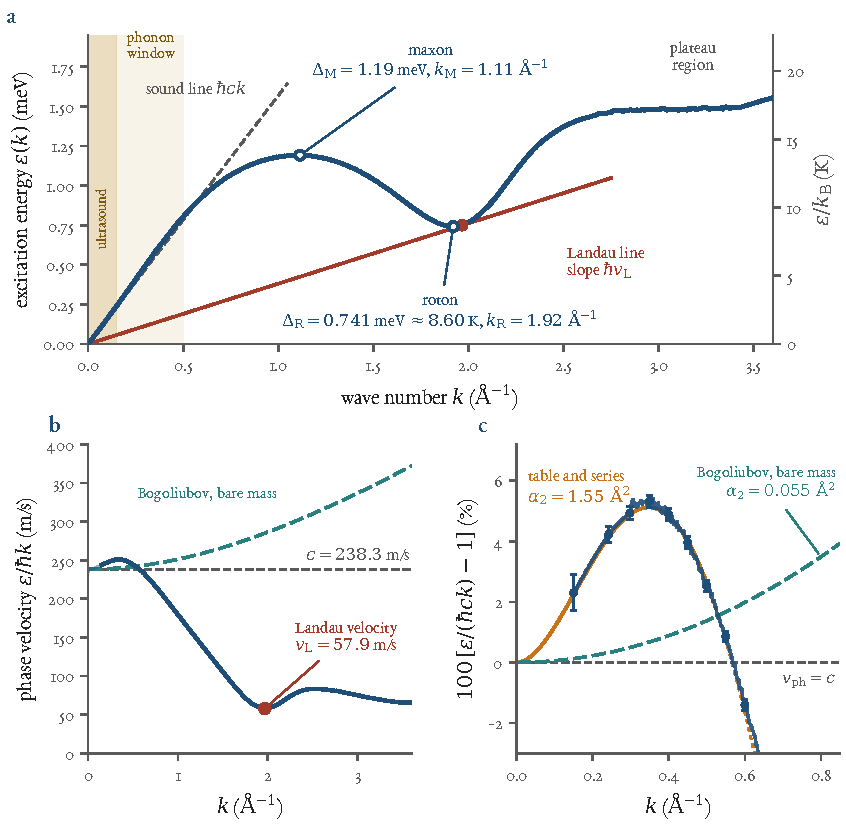
\includegraphics[width=\linewidth]{figures/ch05_curve.pdf}
\caption[The dispersion relation of superfluid helium-4 at saturated vapour pressure]{\textbf{The dispersion relation of superfluid $^4$He at saturated vapour pressure}, from the authors' processed table that accompanies Godfrin \emph{et al.}\ \cite{Godfrin2021} (arXiv ancillary file; not raw counts).
\textbf{a}, $\varepsilon(k)$ with the sound line $\hbar ck$ (grey, $c=\cfiveV{c}\ \mathrm{m\,s^{-1}}$) and the Landau line through the origin that touches the curve at the roton (red; its slope is $\hbar v_{\mathrm L}$).
Open circles: the maximum (maxon) and the minimum (roton) of the table.
The strip below $0.15\ \cfiveAng^{-1}$ is, according to the caption of the paper's own table, ultrasound data; $0.15$--$0.3\ \cfiveAng^{-1}$ combines ultrasound and neutrons; above $0.3\ \cfiveAng^{-1}$ the values are neutron data.
\textbf{b}, the phase velocity $\varepsilon/\hbar k$.
Landau's critical velocity is its minimum, $\cfiveV{landauV}\ \mathrm{m\,s^{-1}}$ at $\cfiveV{landauK}\ \cfiveAng^{-1}$, i.e.\ $\cfiveV{landauOverC}\,c$.
Teal, dashed: the Bogoliubov formula with the bare atomic mass and the measured $c$, which never goes below $c$.
\textbf{c}, the phonon window, $\varepsilon/(\hbar ck)-1$ in per cent: table (with the uncertainties the file gives), the quartic series of \cref{ch05:eq-series} (orange; solid inside its stated range $k<0.5\ \cfiveAng^{-1}$) and the same Bogoliubov curve (teal).
The phase velocity exceeds $c$ by up to $\cfiveV{phaseMaxPct}$ per cent near $\cfiveV{phaseMaxK}\ \cfiveAng^{-1}$.
Script: \texttt{figures/ch05\_curve.py}.}\label{ch05:fig-curve}
\end{figure}

The curve does three things that no free particle does.
For small $k$ it is a straight line, $\varepsilon=\hbar ck$, with the sound speed $c$ that ultrasonics measures: these are the \emph{phonons}.
Near $\cfiveV{maxonKshort}\ \cfiveAng^{-1}$ it turns over at a maximum of about $\cfiveV{maxonE}$ meV, the \emph{maxon}.
It then falls to a minimum of $\cfiveV{rotonE}$ meV --- $\cfiveV{rotonGapK}$ kelvin --- at $\cfiveV{rotonKshort}\ \cfiveAng^{-1}$, the \emph{roton}, and climbs again to a flat shoulder.
Landau proposed a spectrum of this kind in 1941 and, in 1947, corrected it to a single curve in which phonons and rotons are the two ends of one dispersion relation \cite{Landau1941,Landau1947}.
The name is historical: no rotation takes place, and the Godfrin--Krotscheck review describes the minimum as the sign of an incipient short-range order that ends, under enough pressure, in solid helium \cite{GodfrinKrotscheck2022}.
According to the same review, Feynman and Cohen suggested inelastic neutron scattering as the way to see the curve \cite{FeynmanCohen1956}, and the first evidence for the roton minimum came from cold neutrons in 1957 \cite{Palevsky1957}.

\begin{godfrinbox}{What was measured}
\textbf{Experiment.} Inelastic neutron scattering on superfluid $^4$He at the ILL spectrometer IN5, giving the dispersion relation of the Landau elementary excitations (phonon--maxon--roton) from the smallest wave numbers reachable up to a few $\cfiveAng^{-1}$ \cite{Godfrin2021}.\par\vspace{2pt}
\textbf{What the authors did with it.} They derived the thermodynamic consequences of the measured curve; their Eq.~(22) is the specific-heat series of \cref{ch04}.\par\vspace{2pt}
\textbf{What this chapter does with it.} It reads the published curve (the open table of the arXiv version) as data, and asks which statements about excitations are \emph{kinematic}, that is, consequences of the shape of the curve alone. The Lean library proves several of them as mathematics; the solver shows a different dispersion relation, Bogoliubov's, obeying the same statements.
\end{godfrinbox}

A word on what the table is.
It is the authors' own processed curve, not a list of raw counts; the raw data are a different object, and nothing in this book depends on them.
Its composition matters for what can be inferred from it, and the caption of the table in the arXiv version says so: below $0.15\ \cfiveAng^{-1}$ the entries are ultrasound data, from $0.15$ to $0.3\ \cfiveAng^{-1}$ ultrasound and neutron data are combined, and above $0.3\ \cfiveAng^{-1}$ they are neutron data.
The printed version of the table quotes uncertainties of $0.001$ to $0.002$ meV for $k$ between $0.2$ and $2\ \cfiveAng^{-1}$.
(This chapter quotes the arXiv version throughout; it has not been compared with the journal version of record.)

\subsection*{From arrival times to energies}
How does one get from the clock of a detector to a point on the curve?
The incident neutrons have a known energy $E_i$.
For each detector angle one records the time $t_{\rm el}$ at which elastically scattered neutrons arrive (the aluminium of the cell does the elastic scattering; helium scatters none), and the time $t_{\rm in}$ of the helium peak.
If $t_s$ is the moment at which the neutron reaches the sample, the energy lost to the excitation is
\begin{equation}\label{ch05:eq-tof}
 \varepsilon = E_i\Bigl[1-\Bigl(\frac{t_{\rm el}-t_s}{t_{\rm in}-t_s}\Bigr)^{2}\Bigr],
\end{equation}
which is Eq.~(13) of the arXiv version of the paper; the wave number follows from the scattering angle.
Its companion, Eq.~(12), expresses the same energy through the flight distance $D$ and the two arrival times, $\varepsilon=\tfrac12 m_n D^2\,[\,(t_{\rm el}-t_s)^{-2}-(t_{\rm in}-t_s)^{-2}]$, and the two are one formula once $D=v_i(t_{\rm el}-t_s)$ and $E_i=\tfrac12 m_nv_i^2$ are used.
That is a one-line algebraic fact, and it is proved in the Lean library of this programme \cite{Callens2026lib}: \Lthm{HeliumKinematics}{tof_eq12_eq_eq13}.
The analysis therefore rests on two instrumental parameters only ($E_i$ and $t_s$), which is why the energy scale could be fixed \emph{at one point}: the authors calibrated it at the roton, using the value $\Delta_{\rm R}=0.7418\pm0.001$ meV that a triple-axis spectrometer had given, and they remark that if a better roton gap becomes available the energies should be corrected proportionally.
Equation~\eqref{ch05:eq-tof} shows why proportionally: at fixed arrival times, changing $E_i$ by a factor $\lambda$ changes every $\varepsilon$ by the same factor, which the library states as \Lthm{HeliumKinematics}{tofEnergy_rescale}.

It is worth saying how small the quantities are that the next sections will use, because that is what the measurement achieved.
At $k=0.3\ \cfiveAng^{-1}$ the bending of the phonon branch lifts the energy by only $\cfiveV{bend03ueV}$ micro-electronvolts above the sound line, and the excess that decides the three-phonon channel (\cref{ch05:sec-decays}) is at most $\cfiveV{symMax}$ micro-electronvolts.
At the incident energy used for the low wave numbers the energy resolution of the spectrometer is $\cfiveV{resFWHM}$ meV (full width at half maximum) according to the paper \cite{Godfrin2021}: the effects are a third and a fifth of the width of a single line, and the table quotes an uncertainty of $\cfiveV{err03ueV}$ micro-electronvolt near this wave number.
Two things make that possible, both stated in the paper: the resolution function is well described by a Gaussian, so that the centre of a line can be found to a small fraction of its width, and the analysis fits the lines pixel by pixel on a detector of $384$ tubes with $241$ pixels each, averaging typically more than $\cfiveV{nPixBin}$ values into each tabulated wave-number bin.
A curve whose interesting features are a fraction of the width of the instrument's line is a curve that has been measured with great care, not read off.

Two consequences, one practical and one structural, are worth stating before any physics is done.
The practical one: the roton gap of the table ($\cfiveV{rotonE}$ meV at the minimum of the curve; the calibration input was $0.7418$ meV) is tied to the calibration, so it cannot be read as an independent measurement.
The structural one: whatever one concludes from the curve that does not change when $\varepsilon\to\lambda\varepsilon$ is immune to the largest systematic uncertainty of the experiment.
Zero crossings of energy differences, such as those of \cref{ch05:sec-decays}, are of that kind.

\begin{keybox}[The shape decides]
Every statement of this chapter that is a theorem concerns the \emph{shape} of the curve $\varepsilon(k)$: whether it bends up or down away from its tangent at the origin, whether $\varepsilon/\hbar k$ has a minimum below the sound speed, whether $\varepsilon(k_1+k_2)$ exceeds $\varepsilon(k_1)+\varepsilon(k_2)$.
None of them needs a microscopic theory of the liquid, which is why a proof assistant can state them, a published table can be asked for their numerical values, and a simulated field can be tested against them.
\end{keybox}

%% ====================================================================================================================
\section{Landau's reading of the curve}\label{ch05:sec-landau}

Why does the shape of this curve matter so much?
Because it decides whether the liquid is a superfluid.
Landau's argument fits in a paragraph.
Let a heavy body move through the liquid at velocity $\mathbf V$, the liquid being at rest and at zero temperature.
The body can only slow down by creating an excitation of the liquid, of momentum $\hbar\mathbf k$ and energy $\varepsilon(k)$.
Conservation of energy and momentum, with the body so heavy that its recoil energy is negligible, demands $\varepsilon(k)=\hbar\mathbf k\cdot\mathbf V$, which has a solution only if $V\ge\varepsilon(k)/\hbar k$ for some $k$.
Below
\begin{equation}\label{ch05:eq-landau}
 v_{\rm L}=\min_{k>0}\frac{\varepsilon(k)}{\hbar k}
\end{equation}
no excitation can be created and the body moves without friction.
The critical velocity of Landau is the \emph{smallest value of the phase velocity}.

For a gas of free particles, $\varepsilon=\hbar^2k^2/2m$, the phase velocity $\hbar k/2m$ tends to zero with $k$, so $v_{\rm L}=0$: an ideal Bose gas is not a superfluid.
The library proves exactly this, in the form in which it is used: for every $v>0$ there is a wave number at which $a k^2/k<v$ (\Lthm{HeliumKinematics}{landau_velocity_parabolic_zero}).
The same statement from the other side: if the dispersion lies on or above the sound line $ck$, then every phase velocity is at least $c$, so $v_{\rm L}\ge c$ (\Lthm{HeliumKinematics}{landau_velocity_ge_of_above_sound_line}).
A linear start is therefore essential, and a curve that dips \emph{below} the sound line must have a critical velocity below $c$.
Helium does dip below it: \cref{ch05:fig-curve}b shows the phase velocity of the table rising a little above $c$, peaking at $\cfiveV{phaseMaxPct}$ per cent above the ultrasonic value (normalising instead by the $\cfiveV{vphLow}$ m/s that the table itself gives at $0.01\ \cfiveAng^{-1}$ would make it $\cfiveV{phaseMaxPctAlt}$ per cent: the first rows are rounded to $0.1$ micro-electronvolt, so the table fixes $c$ only to a few tenths of a per cent), and then falling nearly linearly to a minimum
\begin{equation}
 v_{\rm L}^{\rm table}=\cfiveV{landauV}\ \mathrm{m\,s^{-1}}=\cfiveV{landauOverC}\,c\qquad\text{at } k=\cfiveV{landauK}\ \cfiveAng^{-1},
\end{equation}
just beyond the roton: the Landau line of \cref{ch05:fig-curve}a is the chord from the origin that touches the curve from below.
If the roton is approximated by Landau's own quadratic form, $\varepsilon\simeq\Delta_{\rm R}+\hbar^2(k-k_{\rm R})^2/2\mu_{\rm R}m_4$, the minimisation can be done in closed form (Exercise~1); with $\mu_{\rm R}=\cfiveV{rotonMass}$ and the gap and wave number of the table it gives $\cfiveV{landauQuad}\ \mathrm{m\,s^{-1}}$, within $\cfiveV{landauQuadPct}$ per cent of the table value.

The seven-pressure table that accompanies the paper allows the same computation under pressure (\cref{ch05:tab-pressure}).
As the pressure rises to $\cfiveV{pP24}$ bar the roton deepens ($\Delta_{\rm R}$ falls to $\cfiveV{pRoton24}$ meV) and moves outward ($k_{\rm R}$ rises to $\cfiveV{pKR24}\ \cfiveAng^{-1}$) while the sound speed rises by $\cfiveV{pCrise}$ per cent, to $\cfiveV{pC24}$ m/s; the Landau velocity therefore \emph{falls}, from $\cfiveV{pLandau0}$ to $\cfiveV{pLandau24}$ m/s, and its ratio to the sound speed is nearly halved, from $\cfiveV{pRatio0}$ to $\cfiveV{pRatio24}$.
The sound speed, which is the Landau velocity of a weakly interacting superfluid and in any case an upper bound for it, grows with the density of the liquid; the quantity that actually sets the ceiling in helium, the roton, moves the other way.
% generated by ch05_numbers.py from the 7-pressure ancillary table
\begin{table}[tp]\centering\small
\begin{tabular}{rrrrrr}\toprule
$P$ (bar) & $c$ (m/s) & $\Delta_{\rm R}$ (meV) & $k_{\rm R}$ ($\text{\AA}^{-1}$) & $v_{\rm L}$ (m/s) & $v_{\rm L}/c$ \\\midrule
0.00 & 238.3 & 0.7413 & 1.920 & 57.9 & 0.243 \\
0.51 & 242.6 & 0.7381 & 1.924 & 57.5 & 0.237 \\
1.02 & 246.5 & 0.7357 & 1.920 & 57.2 & 0.232 \\
2.01 & 253.9 & 0.7301 & 1.932 & 56.5 & 0.223 \\
5.01 & 274.0 & 0.7138 & 1.966 & 54.8 & 0.200 \\
10.01 & 302.3 & 0.6882 & 1.982 & 52.0 & 0.172 \\
24.08 & 361.9 & 0.6256 & 2.048 & 46.1 & 0.127 \\
\bottomrule\end{tabular}
\caption{\textbf{The Landau velocity against pressure}, from the seven-pressure table that accompanies the paper (neutron data from $0.15\ \text{\AA}^{-1}$ to about $\cfiveV{pKmaxRange}\ \text{\AA}^{-1}$). $c$ is the ultrasonic sound velocity quoted in the paper; $\Delta_{\rm R}$ and $k_{\rm R}$ are the minimum of the tabulated curve; $v_{\rm L}=\min_{k>1\,\text{\AA}^{-1}}\varepsilon/\hbar k$ always lies inside the tabulated range. The sound speed rises by $\cfiveV{pCrise}$ per cent over this pressure range while the Landau velocity falls.}\label{ch05:tab-pressure}
\end{table}


One caution, in the spirit of this book.
Equation~\eqref{ch05:eq-landau} is the threshold of one process, the creation of a single elementary excitation.
It does not claim that every flow of $^4$He is dissipationless up to $v_{\rm L}$: a flow can become dissipative earlier by other routes, the nucleation of vortices above all, which is the subject of \cref{ch03,ch06,ch09}.
What the table does give is the \emph{ceiling}, and its value is set by the roton and not by the sound speed.

%% ====================================================================================================================
\section{Three ways a phonon can fail to live}\label{ch05:sec-decays}

\subsection{The sign of the curvature}
At low wave number the curve is written as a series about the sound line,
\begin{equation}\label{ch05:eq-series}
 \varepsilon(k)=\hbar ck\,\bigl(1+\alpha_2k^2+\alpha_3k^3+\alpha_4k^4+\cdots\bigr),
\end{equation}
with no linear term, $\alpha_1=0$ \cite{Godfrin2021}.
At saturated vapour pressure the ultrasonic measurement of Rugar and Foster gives $\alpha_2=1.55\pm0.01\ \cfiveAng^{2}$ when $\alpha_1$ is taken to vanish \cite{RugarFoster1984}, and the paper uses $\alpha_2=1.55\ \cfiveAng^2$, $\alpha_3=-4.04\ \cfiveAng^3$ and $\alpha_4=2.30\ \cfiveAng^4$ to describe the curve for $k<0.5\ \cfiveAng^{-1}$.
In the paper's notation $\alpha_2=-\gamma$, so positive $\alpha_2$ is \emph{anomalous} dispersion: the curve bends upward away from the sound line, as in the first part of \cref{ch05:fig-curve}c.

Anomalous dispersion has a kinematic meaning.
A phonon of wave number $k_1+k_2$ may split into two collinear phonons of wave numbers $k_1$ and $k_2$ only if the energy it gives up is at least what the two products carry, $\varepsilon(k_1+k_2)\ge\varepsilon(k_1)+\varepsilon(k_2)$.
For the straight line $\varepsilon=\hbar ck$ this holds with equality at every $k_1,k_2$: the decay is exactly resonant, and the first correction decides.
With $\varepsilon=\hbar ck(1+ak^2)$, $\hbar=1$, the library has the identity and the equivalence that settle it:

\begin{leanbox}{HeliumKinematics}
\begin{lstlisting}[style=lean]
def phononDisp (c a k : ℝ) : ℝ := c * k * (1 + a * k ^ 2)

theorem three_phonon_open_iff {c a k₁ k₂ : ℝ} (hc : 0 < c) (h₁ : 0 < k₁) (h₂ : 0 < k₂) :
    phononDisp c a k₁ + phononDisp c a k₂ ≤ phononDisp c a (k₁ + k₂) ↔ 0 ≤ a
\end{lstlisting}
\end{leanbox}

The idea of the proof is two lines.
The energy excess of the decay is
$\varepsilon(k_1{+}k_2)-\varepsilon(k_1)-\varepsilon(k_2)=3ca\,k_1k_2(k_1+k_2)$ (\Lthm{HeliumKinematics}{three_phonon_excess}, proved by \texttt{ring}), and for positive $c,k_1,k_2$ the prefactor is positive, so the sign of the excess is the sign of $a$.
This is the statement behind the remark of the paper that phonon damping by three-phonon processes is possible up to a critical wave number when the dispersion is anomalous, and why it disappears at high pressure: the authors report that the dispersion becomes normal, $\alpha_2\le0$, at about $20$ bar \cite{Godfrin2021}, and for normal dispersion the equivalence says the channel is closed.
What it proves is the \emph{mathematical} implication, for the model $\varepsilon=\hbar ck(1+ak^2)$; the sign of $a$ in helium is measured, not proved.

\subsection{Where the channel closes: three numbers, not one}
The quartic series is good only for $k<0.5\ \cfiveAng^{-1}$, and the decay channel closes inside that range, so the interesting question is \emph{where}.
Here the library earns its place, because each way of asking the question gives a different number, and the three are easy to conflate.
Write $\varepsilon=\hbar ck\,(1+\alpha_2k^2+\alpha_3k^3+\alpha_4k^4)$.
Three identities, each proved by the kernel, give
\begin{align}
 \frac{\varepsilon(k)}{\hbar k}-c &= c\,k^{2}\bigl(\alpha_2+\alpha_3k+\alpha_4k^2\bigr), \label{ch05:eq-vph}\\
 \frac{\mathrm d\varepsilon}{\hbar\,\mathrm dk}-c &= c\,k^{2}\bigl(3\alpha_2+4\alpha_3k+5\alpha_4k^2\bigr), \label{ch05:eq-vg}\\
 \varepsilon(k)-2\varepsilon(k/2) &= c\,k^{3}\bigl(\tfrac34\alpha_2+\tfrac78\alpha_3k+\tfrac{15}{16}\alpha_4k^2\bigr). \label{ch05:eq-split}
\end{align}
The first (\Lthm{HeliumKinematics}{phase_velocity_excess}) says where the curve crosses back through the sound line: $v_{\rm ph}=c$.
The second (\Lthm{HeliumKinematics}{group_velocity_excess}) is the group velocity: a phonon can emit a very soft phonon, the limit $q\to0$ of the split $k\to q+(k-q)$, only while its group velocity exceeds $c$ --- a Cherenkov condition.
The third is the symmetric split $k\to k/2+k/2$, whose energy excess is the last to change sign; its statement is short enough to quote:

\begin{leanbox}{HeliumKinematics}
\begin{lstlisting}[style=lean]
def seriesDisp (c α₂ α₃ α₄ k : ℝ) : ℝ := c * k * (1 + α₂ * k ^ 2 + α₃ * k ^ 3 + α₄ * k ^ 4)

theorem symmetric_split_excess (c α₂ α₃ α₄ k : ℝ) :
    seriesDisp c α₂ α₃ α₄ k - 2 * seriesDisp c α₂ α₃ α₄ (k / 2)
      = c * k ^ 3 * (3 / 4 * α₂ + 7 / 8 * α₃ * k + 15 / 16 * α₄ * k ^ 2)
\end{lstlisting}
\end{leanbox}

\noindent It is a polynomial identity (the proof is \texttt{unfold; ring}), so it holds for \emph{every} choice of coefficients, which is its use: the decay threshold of any set of measured $\alpha_j$ is read off a quadratic.
Each right-hand side of \cref{ch05:eq-vph,ch05:eq-vg,ch05:eq-split} is $c\,k^n$ times a quadratic in $k$, so each threshold is the smaller root of an explicit quadratic.
With the coefficients above they are $k_{\rm g}=\cfiveV{kGroup}$, $k_{\rm sym}=\cfiveV{kSym}$ and $k_{\rm ph}=\cfiveV{kPhase}\ \cfiveAng^{-1}$ (the other roots, near $1\ \cfiveAng^{-1}$, lie far outside the range of the series).

\begin{figure}[tp]
\centering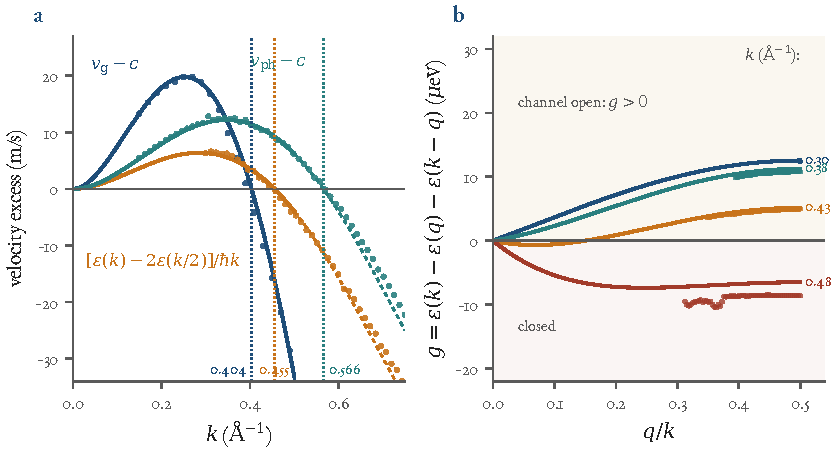
\includegraphics[width=\linewidth]{figures/ch05_thresholds.pdf}
\caption[Where the three-phonon channel closes]{\textbf{Where the three-phonon channel closes.}
\textbf{a}, the three excess velocities of \cref{ch05:eq-vph,ch05:eq-vg,ch05:eq-split} computed from the quartic series (lines; dotted beyond its stated range) and directly from the table (dots; the group velocity is a local linear fit over $\pm0.07\ \cfiveAng^{-1}$).
The zero crossings, in $\cfiveAng^{-1}$, are $\cfiveV{kGroup}$ ($v_{\rm g}=c$, soft emission), $\cfiveV{kSym}$ (symmetric split) and $\cfiveV{kPhase}$ ($v_{\rm ph}=c$).
\textbf{b}, the energy balance $g=\varepsilon(k)-\varepsilon(q)-\varepsilon(k-q)$ of a collinear decay $k\to q+(k-q)$ against $q/k$ for four wave numbers (lines: series; dots: table, where both $q$ and $k-q$ are at least $0.15\ \cfiveAng^{-1}$).
For $k=0.43\ \cfiveAng^{-1}$, between the first and the second threshold, the channel is closed at the soft end and open for near-symmetric splits.
Script: \texttt{figures/ch05\_thresholds.py}.}\label{ch05:fig-thresholds}
\end{figure}

\Cref{ch05:fig-thresholds} shows them, and shows the table agreeing.
Computed straight from the table, without the series, the symmetric split changes sign at $k=\cfiveV{kSymTable}\ \cfiveAng^{-1}$, against $\cfiveV{kSym}$ from the series; the maximum of the excess is $\cfiveV{symMax}$ micro-electronvolts at $\cfiveV{symMaxK}\ \cfiveAng^{-1}$, about three per cent of the energy $\varepsilon(k)$ there, and the series reproduces the table to $\cfiveV{seriesDevMax}$ micro-electronvolts at most for $0.25\le k\le0.5\ \cfiveAng^{-1}$.
This agreement is a consistency check and not an independent confirmation: the coefficients of the series were fitted by the authors to the very curve that the table tabulates.
What it does confirm is the kinematics: the soft end of the channel shuts first, near $\cfiveV{kGroup}\ \cfiveAng^{-1}$, then the symmetric split, and the two should not be mistaken for the sound-line crossing at $\cfiveV{kPhase}\ \cfiveAng^{-1}$, which closes nothing.

The calibration remark of \cref{ch05:sec-curve} pays off here, with a distinction.
The symmetric-split threshold is the zero of a function that is homogeneous of degree one in the energy scale, so it does not move at all if the roton-gap calibration is revised.
The other two compare the curve with the sound speed measured by ultrasonics, and are invariant only if that speed were rescaled with the curve; for a proportional change of the energy scale by the $\cfiveV{relSys}$ that the paper quotes as the relative systematic uncertainty, they move by at most $\cfiveV{shiftG}$ ($k_{\rm g}$) and $\cfiveV{shiftP}\ \cfiveAng^{-1}$ ($k_{\rm ph}$).

\subsection{Two rotons and the plateau}
There is a third kind of decay, with the same logic and a different threshold.
Above the roton the curve flattens into the shoulder that the authors, following the literature, call Pitaevskii's plateau, the energy at which one excitation can decay into two rotons \cite{Godfrin2021,GodfrinKrotscheck2022}.
Two rotons of wave number $k_{\rm R}$ carry a total momentum between $0$ (anti-parallel) and $2k_{\rm R}$ (parallel), so the plateau, which is the locus of the decay, cannot extend beyond $2k_{\rm R}$ in the collinear configuration and can in principle extend down to zero wave number through non-collinear ones, as the review explains \cite{GodfrinKrotscheck2022}.
The geometric core of this is the triangle inequality, and it is a theorem for any inner-product space: \Lthm{HeliumKinematics}{two_roton_momentum_le}, with the extremes attained by \Lthm{HeliumKinematics}{two_roton_parallel} and \Lthm{HeliumKinematics}{two_roton_antiparallel}.
The plateau is not used quantitatively in this book, and nothing is claimed about the data there.

%% ====================================================================================================================
\section{Bogoliubov's phonon, and what it cannot do}\label{ch05:sec-bogoliubov}

\subsection{A phonon that turns into a particle}
There is one quantum fluid in which the whole dispersion relation can be derived on a page, and it is the one the solver simulates.
Take the Gross--Pitaevskii equation with $\hbar=m=1$,
\begin{equation}\label{ch05:eq-gpe}
 \mathrm i\,\partial_t\psi=-\tfrac12\nabla^2\psi+g|\psi|^2\psi ,
\end{equation}
and the uniform solution $\psi_0=\sqrt{n}\,\mathrm e^{-\mathrm i\mu t}$ with $\mu=gn$.
Write $\psi=\mathrm e^{-\mathrm i\mu t}(\sqrt n+\delta)$ and keep terms linear in $\delta$: $\mathrm i\,\partial_t\delta=-\tfrac12\nabla^2\delta+gn(\delta+\delta^*)$.
A plane-wave pair $\delta=u\,\mathrm e^{\mathrm i(kx-\omega t)}+v^*\mathrm e^{-\mathrm i(kx-\omega t)}$ turns this into a two-by-two eigenvalue problem whose determinant gives
\begin{equation}\label{ch05:eq-bog}
 \omega^2=\tfrac12k^2\bigl(\tfrac12k^2+2gn\bigr)\qquad\Longleftrightarrow\qquad
 \varepsilon(k)=\sqrt{c^2\hbar^2k^2+\bigl(\hbar^2k^2/2m\bigr)^2},\quad c^2=\frac{gn}{m},
\end{equation}
the formula Bogoliubov found in 1947 \cite{Bogoliubov1947} (see also \cite{Dalfovo1999,PitaevskiiStringari2016}).
It is a phonon, $\varepsilon\simeq\hbar ck$, below the wave number
\begin{equation}
 k_\ast=\frac{2mc}{\hbar},
\end{equation}
and a free particle, $\varepsilon\simeq\hbar^2k^2/2m$, above it; the wave number $k_\ast$ is the inverse of the healing length of the condensate up to a numerical factor (with $\xi=\hbar/mc$, the convention of the solver, $k_\ast\xi=2$).
The phonon \emph{turns into a particle} as $k$ increases, and the whole curve depends on the single wave number $k_\ast$: for $c,m,k>0$,
\begin{equation}\label{ch05:eq-universal}
 \frac{\varepsilon(k)}{ck}=\sqrt{1+(k/k_\ast)^2}
\end{equation}
(\Lthm{BogoliubovDispersion}{phase_velocity_universal}).
Everything that follows about Bogoliubov's curve is a statement about this one function.
These excitations are waves of density and of phase in a single-valued $\psi$: the velocity they carry, $\hbar\nabla S/m$ for $\psi=\sqrt\rho\,\mathrm e^{\mathrm iS}$, is the gradient of a single-valued phase, so it is irrotational and carries no circulation.
They are the first of the two kinds of excitation of the same field distinguished in \cref{ch03}; the second kind, the vortices, is not in the linearised equation at all.

\subsection{What is proved about it}
Several properties of \cref{ch05:eq-bog} are used below, and each is a theorem in the new Lean module written for this chapter, the file \texttt{Ch05\_\allowbreak BogoliubovDispersion}, whose namespace is \texttt{QuantumFluids.\allowbreak BogoliubovDispersion}; the module is new and is not part of the library \texttt{QuantumFluids}.
Its definitions are the Bogoliubov energy and the curvature coefficient, and its first theorem is the dictionary between the solver's parameters and the formula,
$\varepsilon^2=\tfrac12k^2(\tfrac12k^2+2gn)$ when $c^2=gn$ and $m=1$ (\Lthm{BogoliubovDispersion}{bogEps_sq_gp}), which is the expression the solver's known answer K5 is tested against in \cref{ch05:sec-solver}.
The module proves:
\begin{itemize}
 \item $\varepsilon$ is strictly increasing on $[0,\infty)$ (\Lthm{BogoliubovDispersion}{bogEps_strictMonoOn}): there is no maxon, no roton, no stationary point at all;
 \item $\varepsilon(k_1)+\varepsilon(k_2)<\varepsilon(k_1+k_2)$ for all $k_1,k_2>0$ (\Lthm{BogoliubovDispersion}{bogEps_superadditive}): the collinear decay of a phonon into two is open at \emph{every} wave number, not only below a critical one --- the spectrum is anomalous throughout, in the sense of \cref{ch05:sec-decays}, which is the kinematic precondition of what the literature calls Beliaev damping (its rate is not computed here);
 \item $\varepsilon(k)-ck$ is strictly increasing (\Lthm{BogoliubovDispersion}{bogEps_sub_sound_strictMonoOn}): the energy of an excitation outruns the sound line at every wave number, the derivative-free form of the statement that the group velocity exceeds $c$;
 \item the low-$k$ expansion has the curvature coefficient $\alpha_2=1/(8m^2c^2)$, with the explicit error band below;
 \item the Landau velocity of the spectrum is $c$, exactly.
\end{itemize}
The last two are worth displaying.
The first is the quantitative form of the expansion, a two-sided bound whose proof is the elementary inequality $\sqrt{1+2t}\le1+t$ and its refinement $\sqrt{1+2t}\ge1+t-t^2/2$:

\begin{leanbox}[title={Lean 4 \enspace BogoliubovDispersion (new for this book)}]{BogoliubovDispersion (new)}
\begin{lstlisting}[style=lean]
noncomputable def bogEps (c m k : ℝ) : ℝ := Real.sqrt (c ^ 2 * k ^ 2 + (k ^ 2 / (2 * m)) ^ 2)

noncomputable def alpha2 (c m : ℝ) : ℝ := 1 / (8 * m ^ 2 * c ^ 2)

theorem abs_bogEps_sub_phononDisp_le {c m k : ℝ} (hc : 0 < c) (hm : 0 < m) (hk : 0 ≤ k) :
    |bogEps c m k - phononDisp c (alpha2 c m) k| ≤ c * (alpha2 c m) ^ 2 * k ^ 5 / 2

theorem landau_velocity_eq {c m : ℝ} (hc : 0 < c) (hm : 0 < m) :
    IsGLB ((fun k => bogEps c m k / k) '' Set.Ioi 0) c
\end{lstlisting}
\end{leanbox}

\noindent Here \texttt{phononDisp} is the definition of the library repeated verbatim in the new file, so that the module can be compiled alone.
In words: the Bogoliubov energy differs from $ck(1+\alpha_2k^2)$ by at most $c\alpha_2^2k^5/2$, so the curvature coefficient of the phonon branch is $1/(8m^2c^2)>0$ and the error of the quadratic correction is of order $k^5$ (\Lthm{BogoliubovDispersion}{alpha2_limit} states the limit); and the infimum of the phase velocity $\varepsilon/k$ over $k>0$ is exactly $c$ and is not attained, because $\varepsilon/k=\sqrt{c^2+k^2/4m^2}>c$ at every $k>0$ (\Lthm{BogoliubovDispersion}{sound_lt_phase_velocity}).
By Landau's criterion the critical velocity of this superfluid is therefore its sound speed and nothing less: no excitation of the Bogoliubov spectrum is cheaper per unit momentum than a phonon.
The proof of the upper half of the band is short enough to show, in the form in which it was compiled; the auxiliary identity \texttt{eps\_arg} that it uses ($c^2k^2+(k^2/2m)^2=(ck)^2(1+2\alpha_2k^2)$, by \texttt{field\_simp; ring}) is not shown (proof abridged):

\begin{leanbox}[title={Lean 4 \enspace BogoliubovDispersion (new for this book)}]{BogoliubovDispersion (new)}
\begin{lstlisting}[style=lean]
theorem bogEps_le_phononDisp {c m k : ℝ} (hc : 0 < c) (hm : 0 < m) (hk : 0 ≤ k) :
    bogEps c m k ≤ phononDisp c (alpha2 c m) k := by
  have ha : 0 < alpha2 c m := by unfold alpha2; positivity
  unfold bogEps phononDisp
  rw [Real.sqrt_le_iff]
  refine ⟨by positivity, ?_⟩
  rw [eps_arg hc hm]                       -- (ck)^2 (1 + 2t), t = alpha2 k^2
  have : (c * k) ^ 2 * (1 + 2 * (alpha2 c m * k ^ 2)) ≤ (c * k) ^ 2 * (1 + alpha2 c m * k ^ 2) ^ 2 := by
    apply mul_le_mul_of_nonneg_left _ (sq_nonneg _)
    nlinarith [sq_nonneg (alpha2 c m * k ^ 2)]   -- 1+2t <= (1+t)^2
  calc _ ≤ _ := this
    _ = _ := by ring
\end{lstlisting}
\end{leanbox}

\noindent The lower half is the same argument with $(1+t-t^2/2)^2\le1+2t$, valid when $1+t-t^2/2\ge0$; when that quantity is negative the lower bound is itself negative and holds trivially, because $\varepsilon\ge0$.
All of it was compiled with Lean~4 and Mathlib on the machine that ran the solver, with no \texttt{sorry} and only the three standard axioms.

\subsection{Against helium: how far is the real curve from the weak-coupling one?}
Bogoliubov's derivation assumes a dilute gas whose interaction can be replaced by one coupling constant.
Liquid helium is neither.
Still the \emph{shape} of \cref{ch05:eq-bog} can be compared with the measured curve with no free parameter, because the formula has only two inputs, the mass and the sound speed, and both are known: the bare mass of the $^4$He atom and $c=\cfiveV{c}\ \mathrm{m\,s^{-1}}$.
With them the wave number of the problem is $k_\ast=2mc/\hbar=\cfiveV{kstar}\ \cfiveAng^{-1}$, which is \emph{inside} the measured range, and the curvature coefficient of the phonon branch is $\alpha_2^{\rm Bog}=1/(2k_\ast^2)=\cfiveV{alphaBog}\ \cfiveAng^2$, against the measured $1.55\ \cfiveAng^2$: the real curve bends away from the sound line \cfiveV{alphaRatio} times faster.
\Cref{ch05:fig-curve}b,c show the comparison; the Bogoliubov phase velocity climbs without limit while the measured one turns over at $k\approx\cfiveV{phaseMaxK}\ \cfiveAng^{-1}$ and falls to a quarter of $c$.

The two-sided reading is the point of this book's rule about analogies.
The comparison measures \emph{how far helium is from the hypotheses that Bogoliubov's formula needs}; it does not test the formula, which is a theorem about the Gross--Pitaevskii equation, and it does not say that a gas with those parameters would behave like helium.
A property that the roton depends on is not a property of the Gross--Pitaevskii equation with a contact interaction: a monotonically increasing $\varepsilon$ has no minimum, whatever the value of $g$.
The roton needs structure on the scale of the interatomic distance.
Feynman's account is that the energy of the excitation is, at best, $\hbar^2k^2/2mS(k)$, with $S(k)$ the static structure factor, and that this is an \emph{upper bound} to the true excitation energy \cite{Feynman1954,FeynmanCohen1956}; the minimum of $\varepsilon$ sits where $S(k)$ has its first peak, the signature of the short-range order of the liquid.
In the weak-coupling theory $S(k)=(\hbar^2k^2/2m)/\varepsilon(k)$ and the bound is saturated; in helium it is not, and the paper itself remarks that the Bijl--Feynman spectrum is ``clearly very far from the experimental result'' \cite{Godfrin2021}.

A different mechanism produces a roton minimum in a Bose gas, and the difference is the lesson of this section.
Give the atoms a non-local interaction whose Fourier transform $V(k)$ becomes negative in a window, as for dipolar atoms, and the Bogoliubov spectrum becomes $\omega^2=\epsilon_k(\epsilon_k+2nV(k))$ with $\epsilon_k=\hbar^2k^2/2m$: it can have a roton minimum, and such rotons have been seen in a dipolar quantum gas \cite{Santos2003,Chomaz2018}.
That is a mean-field roton produced by the sign of an interaction in $k$-space; the helium roton is the signature of short-range order.
The two share a name and a shape, and the properties that depend on the mechanism --- what the roton mass is, how it responds to pressure, what it does at the liquid--solid transition --- are not transferable from one to the other without checking (Exercise~3).


%% ====================================================================================================================
\section{The solver as a spectrometer}\label{ch05:sec-solver}

The projected Gross--Pitaevskii equation is the one quantum fluid of this book whose dispersion relation is known in closed form, and that makes it a test bench: if the excitations of the simulated field do not obey \cref{ch05:eq-bog}, the instrument is wrong.
The instrument is \texttt{qf-pgpe}, the Rust engine of rusty-SUNDIALS that \cref{ch02} describes.
It integrates $\mathrm i\,\partial_t\psi=P[-\tfrac12\nabla^2\psi+g|\psi|^2\psi]$ on a doubly periodic box with an integrating-factor fourth-order Runge--Kutta step (the linear part exact, the cubic part by RK4) and a sharp circular cutoff $P$ at $k_{\rm cut}=k_{\max}/2$, which is the condition under which the cubic term does not alias into the retained modes.
The crate's own documentation records agreement with the numpy engine of the programme to $10^{-10}$ over twenty time units \cite{Callens2026sw}.
Units are $\hbar=m=n_0=1$ and $g=1$, so that $c=1$, $\xi=\hbar/mc=1$ and $k_\ast=2$.
The box is $L=64\,\xi$ on a $128\times128$ grid, which retains \cfiveV{nmodesRetained} wave vectors with $|k|\le\pi/\xi$.

\subsection{Exciting every mode at once}
A time-of-flight spectrometer covers hundreds of scattering angles at once, and the simulation can do the same.
Start from the uniform condensate $\psi=1$ and add a weak random complex amplitude, of size $\eta=10^{-6}$, to \emph{every} retained mode; evolve for $T=\cfiveV{Tmain}$; every $0.4$ time units record the amplitude $c_k(t)$ of every mode.
In the linear regime each mode then oscillates as a superposition of the two normal modes of the pair $\pm k$, so that, with the proper frame (next paragraph),
\begin{equation}\label{ch05:eq-twofreq}
 s_k(t)=\alpha_k\,\mathrm e^{-\mathrm i\omega_kt}+\beta_k\,\mathrm e^{+\mathrm i\omega_kt},
\end{equation}
two complex amplitudes and one frequency per mode.
For each mode the frequency is the value of $\omega$ that minimises the residual of the best linear fit of the two amplitudes; the residual is evaluated in closed form, and a golden-section search, started from a one-step linear-prediction estimate, finds the minimum in \cfiveV{nGolden} evaluations.
The half-records give a model-free error proxy: the two halves of the record are fitted separately and the difference is reported.
One run yields \cfiveV{nModesMain} measurements of the dispersion relation.

\subsection{The frame lesson}
The record is kept in the \emph{condensate frame}, $s_k=c_k\,c_0^\ast/|c_0|$, where $c_0$ is the amplitude of the $k=0$ mode, and the reason is an episode that the programme recorded as a failure.
In its pre-registered list of known answers for the engine, the Bogoliubov test (called K5) failed at the first attempt, by factors of $5$, $2.5$ and $1.2$ in the frequency, before any physics was run \cite{Callens2026prereg}.
The cause was not the engine.
The equation has no chemical potential in it, so the condensate rotates in the laboratory frame as $\mathrm e^{-\mathrm i\mu t}$ with $\mu=gn_0$, and every mode amplitude inherits that phase: the measured frequencies were $\mu\pm\omega$.
The record of this run shows it directly.
For the mode $(16,0)$, $k=\cfiveV{labK}$, the Bogoliubov frequency is $\omega=\cfiveV{labOmega}$, and the laboratory-frame record has its two spectral peaks at $\cfiveV{labPeakA}$ and $+\cfiveV{labPeakB}$, which are $-(\mu+\omega)=\cfiveV{labExpA}$ and $-\mu+\omega=+\cfiveV{labExpB}$ to within the $10^{-3}$ resolution of the peak position.
Reading the larger peak as the excitation frequency gives about $3$ where the answer is $2$; reading the smaller gives about $1$.
Dividing by the condensate's phase fixed the test.
The same logic holds for the experiment: a neutron's energy loss $E_i-E_f$ is measured against the ground state of the liquid, and the chemical potential of the liquid never appears.
A frequency is a statement about a frame.

\begin{rustbox}{the broadband pulse and the condensate frame}
\begin{lstlisting}[style=py,basicstyle=\ttfamily\footnotesize]
import numpy as np, qf_pgpe
eng = qf_pgpe.Pgpe(N, L, g, dt, 0.5)             # n, L, g, dt, k_cut/k_max

def initial_pulse(eng, N, eta, seed):                 # (docstring removed)
    rng = np.random.default_rng(seed)
    mask = mode_set(eng, N)
    c = np.array(eng.uniform(), dtype=complex)
    xi = (rng.normal(size=(N, N)) + 1j * rng.normal(size=(N, N))) / np.sqrt(2.0)
    add = eta * N ** 2 * xi * mask
    add[0, 0] = 0.0
    return c + add, mask

def record_condensate_frame(run_step, c0, mask, n_samples, N, keep_lab=None):
    c = c0                                            # (docstring removed)
    nm = int(mask.sum())
    out = np.empty((n_samples, nm), dtype=np.complex128)
    lab = np.empty(n_samples, dtype=np.complex128) if keep_lab is not None else None
    for j in range(n_samples):
        if j > 0:
            c = run_step(c)                       # eng.run(c, 0.4): 20 steps
        c = np.asarray(c)
        ph = np.conj(c[0, 0]) / abs(c[0, 0])  # condensate frame: remove exp(-i mu t)
        out[j] = c[mask] * ph / N ** 2
        if lab is not None:
            lab[j] = c[keep_lab] / N ** 2
    return out, lab
\end{lstlisting}
\end{rustbox}

The code is the code that was run (\cfivepath{figures/ch05_common.py}; the main run is \cfivepath{figures/ch05_dispersion_run.py}).
The main run, $15\,000$ steps of a $128^2$ grid, took \cfiveV{secRun} seconds of wall time, plus \cfiveV{secFit} seconds of fitting, on the shared eight-core machine of this project while its load average was between ten and thirty-six; the figure is indicative of the order of magnitude and not a benchmark.

\subsection{What the measurement shows}
\begin{figure}[tp]
\centering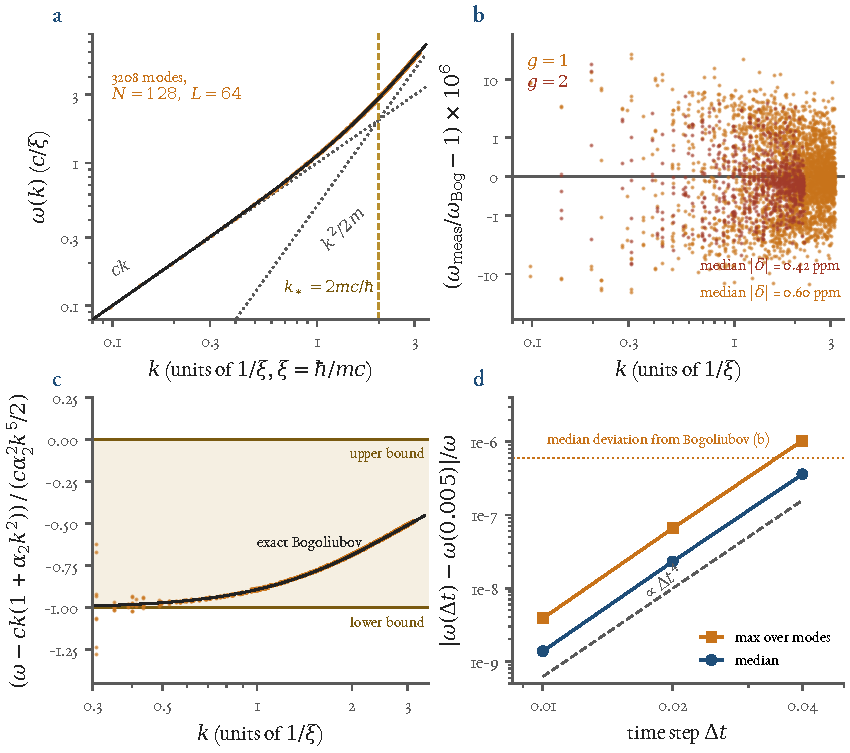
\includegraphics[width=\linewidth]{figures/ch05_solver.pdf}
\caption[The solver measures Bogoliubov's dispersion relation]{\textbf{The solver measures Bogoliubov's dispersion relation.}
\textbf{a}, the frequencies of all \cfiveV{nModesMain} modes of the $128^2$ run (orange) on the Bogoliubov curve (black) between its two asymptotes (dotted).
\textbf{b}, the relative deviation of every mode from $\omega_{\rm Bog}$, in parts per million, for $g=1$ and for a second run with $g=2$ ($c=\sqrt2$; the wave number is in units of $1/\xi=mc/\hbar$).
\textbf{c}, the band proved in Lean: the quantity $(\omega-ck(1+\alpha_2k^2))/(c\alpha_2^2k^5/2)$ lies in $[-1,0]$ for the Bogoliubov spectrum, and the measured points follow the exact curve (black) from the lower edge, which is asymptotically sharp as $k\to0$.
Below $k\approx0.5$ the noise of the fit, magnified by the $k^{-5}$ of the normalisation, takes some points out of the band; the band is a theorem about the formula, the points are measurements.
\textbf{d}, the time-step ladder: differences between the frequencies obtained with $\Delta t=0.04$, $0.02$, $0.01$ and those of the same pulse with $\Delta t=0.005$; they fall by a factor $\cfiveV{ratioA}$ and then $\cfiveV{ratioB}$ per halving, the fourth-order law of the scheme.
Script: \texttt{figures/ch05\_dispersion\_run.py} (data), \texttt{figures/ch05\_solver\_fig.py} (figure).}\label{ch05:fig-solver}
\end{figure}

\Cref{ch05:fig-solver}a shows the result: all \cfiveV{nModesMain} frequencies, over almost a decade and a half in $k$, lie on Bogoliubov's curve, bending from the sound line to the free-particle parabola across $k_\ast$.
The deviations (\cref{ch05:fig-solver}b) have a median of $\cfiveV{medMain}$ parts per million, $99$ per cent of the modes are within $\cfiveV{p99Main}$ ppm and the worst is $\cfiveV{maxMain}$ ppm.
The error is not uniform in $k$: the median is $\cfiveV{medLowK}$ ppm below $k=0.4$ and $\cfiveV{medHighK}$ ppm above $k=2.5$, because the slowest modes complete only a few periods in the record; the half-record difference, which is blind to the model, has a median of $\cfiveV{medSplit}$ ppm and says the same.
So this is a statement about the fit as much as about the engine, and it is a good one: the engine's frequencies equal the closed form to a few parts in $10^7$.

Three further checks sit in the same figure.
The second run, with $g=2$, gives a median of $\cfiveV{medG2}$ ppm over $\cfiveV{nModesG2}$ modes: the dictionary $c^2=gn_0$ of \Lthm{BogoliubovDispersion}{bogEps_sq_gp} is right.
The Lean theorem \Lthm{BogoliubovDispersion}{abs_bogEps_sub_phononDisp_le} meets data in the band of \cref{ch05:fig-solver}c: for the $\cfiveV{nBand}$ modes with $k\ge0.5$ all of the points lie inside $[-1,0]$, between $\cfiveV{zMin}$ and $\cfiveV{zMax}$, and the largest distance from the exact curve is $\cfiveV{zDev}$ in these units.
The ladder of \cref{ch05:fig-solver}d is the integrator's own order: the median difference to the finest run is $\cfiveV{ladA}$, $\cfiveV{ladB}$ and $\cfiveV{ladC}$ for $\Delta t=0.04$, $0.02$, $0.01$, a drop of $\cfiveV{ratioA}$ and $\cfiveV{ratioB}$ per halving.
At the step used for the main run, $\Delta t=0.02$, the time-stepping error is therefore a factor $\cfiveV{ladVsFit}$ smaller than the fit's own scatter.

\subsection{One function of one variable}
\begin{figure}[tp]
\centering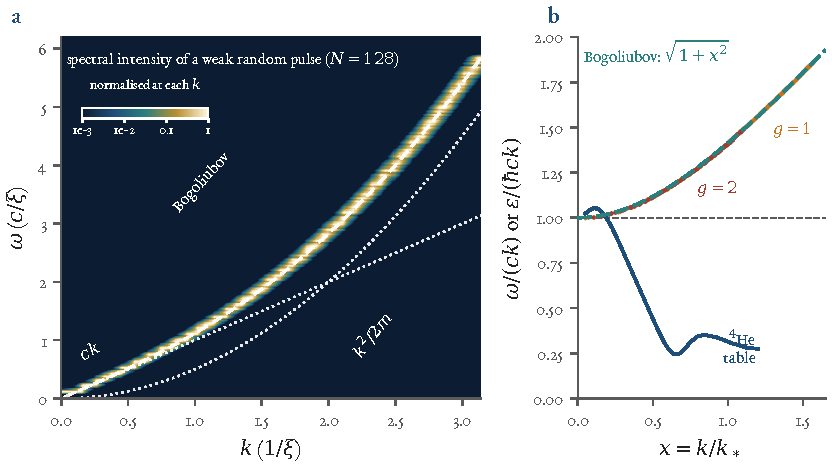
\includegraphics[width=\linewidth]{figures/ch05_universal.pdf}
\caption[A spectrometer map of the simulated fluid, and the universal curve]{\textbf{A spectrometer map of the simulated fluid, and the universal curve.}
\textbf{a}, the power spectrum of the record of every mode, folded onto positive frequency, smeared in $k$ with a Gaussian of width $0.03/\xi$ (a display resolution, like the finite angular resolution of an instrument), and normalised at each $k$.
A bright ridge follows the Bogoliubov curve (white, dashed) from the sound line to the free-particle parabola (dotted).
The intensity along the ridge is set by the random pulse and has no physical meaning; only the position of the ridge does.
\textbf{b}, the phase velocity in units of $c$ against $x=k/k_\ast$, $k_\ast=2mc/\hbar$: the $g=1$ run (orange) and the $g=2$ run (red) fall on the single curve $\sqrt{1+x^2}$ (teal) of \cref{ch05:eq-universal}, to within $\cfiveV{collapseA}$ and $\cfiveV{collapseB}$; the measured curve of $^4$He (blue, with the bare atomic mass and $c=238.3$ m/s in $k_\ast$) leaves it at $x\approx0.1$ and has no part in common with it beyond.
Script: \texttt{figures/ch05\_solver\_fig.py}.}\label{ch05:fig-universal}
\end{figure}

Equation~\eqref{ch05:eq-universal} says that the whole curve is a function of one variable, and the two runs test it.
In the coordinates $x=k/k_\ast$ and $y=\omega/(ck)$ the $g=1$ and the $g=2$ runs, whose sound speeds differ by $\sqrt2$ and whose cutoffs sit at different $x$, collapse on $\sqrt{1+x^2}$ to within $\cfiveV{collapseA}$ and $\cfiveV{collapseB}$ (\cref{ch05:fig-universal}b).
Helium, in the same coordinates with the bare atomic mass, does not: it leaves the universal curve at $x\approx0.1$, rises to $\cfiveV{phaseMaxRatio}$ and falls to $\cfiveV{rotonYat}$ at the roton.
The two curves have the same two inputs and nothing else in common.

\Cref{ch05:fig-universal}a is the same data seen as an experimentalist sees $S(Q,\omega)$: a map in the $(k,\omega)$ plane, with a bright line where the excitations are.
It is, if one likes, a numerical neutron-scattering experiment.
It shows no maxon and no roton, only a ridge that never turns over, and the point of the figure is that contrast: the line a neutron spectrometer draws for helium (\cref{ch05:fig-curve}a) has structure that a contact-interaction Gross--Pitaevskii field cannot produce.
Two caveats keep the analogy honest.
The intensity along the ridge is an artefact of our random pulse; the physical weight of the single-excitation peak is the static structure factor $S(k)=(\hbar^2k^2/2m)/\varepsilon(k)$ of Bogoliubov's theory, and a classical field at zero temperature has no way to produce it.
And the lines of the map are as sharp as the window allows, because the field is integrated for three hundred time units without damping; what limits the width of the excitation peaks in real helium --- the decay channels of \cref{ch05:sec-decays} --- is not computed here.

\subsection{Waves in space: the group velocity}
The frequency of one wave number is one way to see the dispersion; a wave packet is another, and it measures a different quantity, the group velocity.
\begin{figure}[tp]
\centering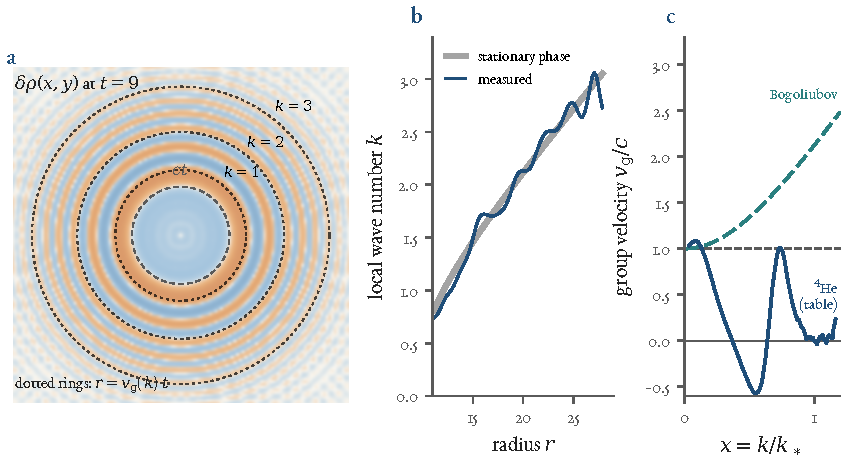
\includegraphics[width=\linewidth]{figures/ch05_rings.pdf}
\caption[A dispersive ring wave]{\textbf{A dispersive ring wave.}
\textbf{a}, the density deviation $\delta\rho$ (symmetric logarithmic colour scale) at $t=9$ after a Gaussian density bump of width $0.6\,\xi$ and height $0.02$ at the centre of the box (zero initial velocity; $128^2$ grid, $L=64\,\xi$, bicubic interpolation for display).
The ring at $r=ct$ is the sound front; outside it the ripples are the short waves that run ahead, each wave number $k$ at the radius $v_{\rm g}(k)\,t$ (dotted circles for $k=1,2,3$).
\textbf{b}, the local wave number of the azimuthally averaged profile (blue; phase of the analytic signal of $\sqrt r\,\delta\rho$) against the stationary-phase prediction $v_{\rm g}(k_s)=r/t$ (grey).
\textbf{c}, the group velocity in units of $c$ against $x=k/k_\ast$: Bogoliubov (teal, dashed) rises monotonically to $\cfiveV{vgKcut}\,c$ at the cutoff; for $^4$He (blue, local linear fit to the table) it reaches only $\cfiveV{vgMax}\,c$ near $\cfiveV{vgMaxK}\ \cfiveAng^{-1}$, vanishes at the maxon ($\cfiveV{vgZeroK}\ \cfiveAng^{-1}$), turns negative ($\cfiveV{vgMin}\,c$ at $\cfiveV{vgMinK}\ \cfiveAng^{-1}$) and returns to zero at the roton.
Script: \texttt{figures/ch05\_rings.py}.}\label{ch05:fig-rings}
\end{figure}
A localised density pulse contains all wave numbers.
Each travels at its own group velocity $v_{\rm g}=\mathrm d\omega/\mathrm dk=(k+k^3/2)/\omega$ (units $c=m=\hbar=1$), so that the stationary-phase argument puts the wave number $k$ at the radius $r=v_{\rm g}(k)\,t$: a snapshot of the density is a map of the dispersion relation read through its derivative.
Since $\varepsilon(k)-ck$ is increasing (\Lthm{BogoliubovDispersion}{bogEps_sub_sound_strictMonoOn}), the mean group velocity between any two wave numbers exceeds $c$, and the ripples run ahead of the front.
\Cref{ch05:fig-rings} shows it.
The local wave number of the ripples, measured in the range $r=\cfiveV{ringRmin}$ to $\cfiveV{ringRmax}\,\xi$ (wave numbers $\cfiveV{ringKmin}$ to $\cfiveV{ringKmax}/\xi$), follows the stationary-phase prediction with a median relative deviation of $\cfiveV{ringMed}$ per cent (largest: $\cfiveV{ringMax}$ per cent at the edges of the window, where the phase of the analytic signal is least reliable).
No fit and no free parameter enters: the dispersion relation has been read off a single snapshot, and it is the same one that was read off $\cfiveV{nModesMain}$ time series.

Panel c is the comparison with the helium of \cref{ch05:sec-curve}, in the universal coordinate $x$.
The group velocity of Bogoliubov's fluid exceeds $c$ at every wave number and grows without bound ($\cfiveV{vgKcut}\,c$ at the cutoff of the simulation).
The group velocity of helium, computed from the table by a local linear fit, rises above $c$ by $\cfiveV{vgMaxPct}$ per cent near $\cfiveV{vgMaxK}\ \cfiveAng^{-1}$ and returns to $c$ at $\cfiveV{vgCrossK}\ \cfiveAng^{-1}$ (the series of \cref{ch05:sec-decays} gives $\cfiveV{kGroup}$); it vanishes at the maxon, is negative between maxon and roton --- excitations whose energy increases while their momentum decreases --- and vanishes again at the roton.
A pulse launched in helium would therefore send ahead of the sound front only the waves with $k$ below about $\cfiveV{vgCrossK}\ \cfiveAng^{-1}$, and the waves between the maxon ($\cfiveV{vgZeroK}\ \cfiveAng^{-1}$) and the roton would travel backwards.
Both statements are consequences of the shape of the table, and neither has been seen in a simulation here, since the engine cannot produce this curve.

\subsection{A referee: CVODE}
The engine is a fixed-step scheme of known order (\cref{ch05:fig-solver}d); an integrator of a different kind is a useful second opinion.
The projected equation is an ordinary differential system for $2n_{\rm modes}$ real numbers, and CVODE, the variable-order solver of rusty-SUNDIALS, integrates it through its Python module \texttt{rusty\_sundials} with the right-hand side supplied from Python.
The interface returns the end state only, so a time series is built by chaining one call per sample interval; the Adams method is the sensible choice for a non-stiff problem.
\begin{rustbox}{the same trajectory under CVODE}
\begin{lstlisting}[style=py,basicstyle=\ttfamily\footnotesize]
# abridged from figures/ch05_cvode.py
from rusty_sundials import CvodeSolver
scale = float(N ** 2)

def rhs(_t, y):                          # dc/dt of the projected GPE; y = (Re c, Im c) / N^2
    c = py.unpack(np.asarray(y) * scale)  # py: numpy engine, same equation, same modes
    return (py.pack(py.rhs(c)) / scale).tolist()

solver = CvodeSolver("adams", rtol, atol, 10_000_000)
y = (py.pack(c0) / scale).tolist()
for j in range(1, ns):
    _, y = solver.solve(rhs, (j - 1) * dts, y, j * dts)   # one call per sample interval
\end{lstlisting}
\end{rustbox}
This cross-check has a history that belongs to the record.
The software paper of the engine makes the same comparison, the engine against a CVODE reference on a box of $16\times16$ points with $49$ modes, and reports that it depends on a fix of the library, ``the Adams order was stuck at one'': without the fix the solver collapses its step on this oscillatory Hamiltonian problem and fails after about $10^6$ right-hand-side evaluations \cite{Callens2026sw}.
The module installed in the project's virtual environment predates the fix (it was installed on \cfiveV{cvOldDate}), and \cref{ch05:tab-cvode-builds} shows the difference from the outside: on a box of $\cfiveV{cvSmallN}\times\cfiveV{cvSmallN}$ points the older build needs $\cfiveV{cvRatio4}$, $\cfiveV{cvRatio6}$ and $\cfiveV{cvRatio8}$ times as many right-hand-side evaluations as the current one at tolerances $10^{-4}$, $10^{-6}$ and $10^{-8}$.
At the same tolerance it is also less accurate (at $10^{-6}$ its frequencies differ from the engine's by $\cfiveV{cvOldErr6}$, those of the current build by $\cfiveV{cvNewErr6}$).
Its cost grows roughly as the inverse square root of the tolerance (by factors of $\cfiveV{cvGrowOldA}$ and $\cfiveV{cvGrowOldB}$ for each hundredfold tightening, where an exact square-root law gives ten) and its error falls by about $\cfiveV{cvOldFallA}$ and $\cfiveV{cvOldFallB}$ over the same steps, which is how a first-order method behaves when the step is set by an error that is quadratic in the step.
The first attempt at this section was run on the older build and was abandoned for that reason; everything below uses the current build.
% generated by ch05_numbers.py from ch05_cvode_new.json / ch05_cvode_old.json
\begin{table}[t]\centering\small
\begin{tabular}{rrrrr}\toprule
tolerance (rtol) & \multicolumn{2}{c}{older build} & \multicolumn{2}{c}{current build}\\
 & right-hand sides & $\max|\Delta\omega|/\omega$ & right-hand sides & $\max|\Delta\omega|/\omega$ \\\midrule
\ensuremath{10^{-4}} & 1\,361 & \ensuremath{1.9\times10^{-2}} & 599 & \ensuremath{3.8\times10^{-4}} \\
\ensuremath{10^{-6}} & 9\,730 & \ensuremath{1.7\times10^{-3}} & 718 & \ensuremath{1.7\times10^{-5}} \\
\ensuremath{10^{-8}} & 91\,519 & \ensuremath{1.7\times10^{-4}} & 992 & \ensuremath{3.5\times10^{-7}} \\
\bottomrule\end{tabular}
\caption{\textbf{The same experiment on two builds of the Python module.} A box of $8^2$ grid points ($13$ modes, $26$ unknowns), $T=4$, the same pulse. The older build is the module of the project's virtual environment (installed on \cfiveV{cvOldDate}); the current one was built from the rusty-SUNDIALS tree (commit 5db8041) that contains the fix of the Adams order.}\label{ch05:tab-cvode-builds}
\end{table}

\begin{table}[t]\centering\small
\begin{tabular}{rrrrr}\toprule
tolerance (rtol) & right-hand sides & wall (s) & $\max|\Delta\omega|/\omega$ & $\max|\Delta s|/|s|$ \\\midrule
\ensuremath{10^{-4}} & 6\,229 & 4.8 & \ensuremath{7.8\times10^{-4}} & \ensuremath{7.7\times10^{-2}} \\
\ensuremath{10^{-6}} & 6\,948 & 5.4 & \ensuremath{2.7\times10^{-5}} & \ensuremath{1.6\times10^{-3}} \\
\ensuremath{10^{-8}} & 8\,313 & 7.0 & \ensuremath{2.7\times10^{-7}} & \ensuremath{1.8\times10^{-5}} \\
\ensuremath{10^{-10}} & 10\,158 & 7.6 & \ensuremath{3.3\times10^{-9}} & \ensuremath{8.0\times10^{-7}} \\
\bottomrule\end{tabular}
\caption{\textbf{CVODE against the Rust engine.} The same random pulse ($\eta=10^{-4}$) on a box of \cfiveV{cvN}$^2$ grid points with \cfiveV{cvModes} retained modes ($\cfiveV{cvUnknowns}$ real unknowns), integrated to $T=\cfiveV{cvT}$ by CVODE's Adams method (atol $=10^{-3}\,$rtol) through the Python interface and by the engine ($\Delta t=0.01$ and a four times smaller step as reference).
Columns: right-hand-side evaluations, wall time on the shared machine, the largest relative difference between the frequencies read from the CVODE record and from the fine-step engine record, and the largest difference between the two mode records, relative to the rms amplitude of each mode.
The engine's own frequencies differ from its four-times-finer run by at most \cfiveV{cvRk4Dt}, and the engine took \cfiveV{cvRustSec} s for this record.
Both records go through the same fit; the frequencies of this short record, in which the modes complete between \cfiveV{cvPerMin} and \cfiveV{cvPerMax} periods, differ from Bogoliubov's formula by up to \cfiveV{cvBogMax}, which cancels in the difference between the two records.}\label{ch05:tab-cvode}
\end{table}

With the current build CVODE does what a referee should (\cref{ch05:tab-cvode}).
The box is that of the software paper's reference, $\cfiveV{cvN}\times\cfiveV{cvN}$ points with $\cfiveV{cvModes}$ modes, integrated here for $\cfiveV{cvT}$ time units.
As the tolerance is tightened from $10^{-4}$ to $10^{-10}$ the frequencies that CVODE gives approach those of the finest run of the engine, the difference falling from $\cfiveV{cvErr4}$ to $\cfiveV{cvErr10}$; the last two rows are below the $\cfiveV{cvRk4Dt}$ by which the engine at its production step differs from that finest run.
The finest run is not exact either: for a scheme of fourth order the error of the run with the four times smaller step is about $1/255$ of that difference, that is $\cfiveV{cvFineErr}$, which is of the order of the last difference, so the comparison cannot resolve more.
Two independent integrators, one of fixed step and fourth order and one of variable order and step, agree on the dispersion relation of the projected equation: the frequencies that the same fit reads from their records differ by $\cfiveV{cvBestErr}$ at most.
What the referee cannot do is scale.
Every right-hand-side evaluation is a call from CVODE into Python, where the numpy engine evaluates the equation and the state is converted to and from a list, and both the number of evaluations and the cost of each one grow with the box: for two time units at tolerance $10^{-6}$ the $\cfiveV{cvScaleUnk8}$-unknown box needs $\cfiveV{cvScale8}$ evaluations and $\cfiveV{cvScaleSec8}$ seconds, the $\cfiveV{cvScaleUnk16}$-unknown box $\cfiveV{cvScale16}$ and $\cfiveV{cvScaleSec16}$ seconds, and the $\cfiveV{cvScaleUnk32}$-unknown box $\cfiveV{cvScale32}$ and $\cfiveV{cvScaleSec32}$ seconds (wall time on the shared machine).
The main run has $\cfiveV{unkMain}$ unknowns, $\cfiveV{unkRatio}$ times as many as the largest box tried here, and was followed for three hundred time units instead of two; it was not attempted through this interface, and for it the evidence is the closed-form reference of \cref{ch05:fig-solver}.
CVODE stays what the software paper made it, an independent reference on small systems and a regression guard for the library.

\subsection{Amplitude: the dispersion relation is a small-amplitude statement}
Everything above is at the amplitude $\eta=10^{-6}$.
The same engine, started from a single standing wave $\psi=1+\epsilon\cos kx$ and read in the same way, shows the limit of the concept.
For the mode $k=\cfiveV{ampK2}/\xi$ the relative frequency shift is $\cfiveV{ampS1}$, $\cfiveV{ampS2}$ and $\cfiveV{ampS3}$ at $\epsilon=0.01$, $0.1$ and $0.3$: it is quadratic in the amplitude, negative (the frequency softens), and reaches $\cfiveV{ampS3pct}$ per cent at $\epsilon=0.3$.
For the longest mode of that run, $k=\cfiveV{ampK1}/\xi$, the two-frequency description of \cref{ch05:eq-twofreq} fails already at $\epsilon=0.1$ (residual $\cfiveV{ampR1}$ of the signal): a nearly dispersionless wave drives its own harmonics nearly resonantly and the single-frequency picture does not survive, which is plausible but has not been tested further here.
The dispersion relation $\omega(k)$ is the $\epsilon\to0$ limit of a family, and the measurements above are taken in that limit.

\begin{table}[tp]
\centering\small
\begin{tabular}{p{0.38\linewidth}p{0.37\linewidth}p{0.14\linewidth}}\toprule
check & result & where\\\midrule
frequencies of all modes against Bogoliubov's formula ($g=1$) & median $\cfiveV{medMain}$ ppm over $\cfiveV{nModesMain}$ modes; worst $\cfiveV{maxMain}$ ppm (lowest $k$) & \cref{ch05:fig-solver}a,b\\
second coupling, $g=2$ & median $\cfiveV{medG2}$ ppm over $\cfiveV{nModesG2}$ modes & \cref{ch05:fig-solver}b\\
collapse on $\sqrt{1+x^2}$ & within $\cfiveV{collapseA}$ ($g=1$) and $\cfiveV{collapseB}$ ($g=2$) & \cref{ch05:fig-universal}b\\
Lean error band, $k\ge0.5$ & all $\cfiveV{nBand}$ modes inside; largest distance from the exact curve $\cfiveV{zDev}$ & \cref{ch05:fig-solver}c\\
order of the time step & differences fall by $\cfiveV{ratioA}$ and $\cfiveV{ratioB}$ per halving (fourth order: $16$) & \cref{ch05:fig-solver}d\\
group velocity from a snapshot & median $\cfiveV{ringMed}$ per cent over $k=\cfiveV{ringKmin}$--$\cfiveV{ringKmax}/\xi$ & \cref{ch05:fig-rings}b\\
CVODE against the engine & at rtol $\cfiveV{cvBestTol}$: frequencies within $\cfiveV{cvBestErr}$, records within $\cfiveV{cvBestTraj}$ & \cref{ch05:tab-cvode}\\
\bottomrule
\end{tabular}
\caption{\textbf{The checks of this chapter at a glance.} Each is an agreement between the engine and a closed form or a second integrator; none is a statement about helium.}\label{ch05:tab-checks}
\end{table}

%% ====================================================================================================================
\section{What this establishes, and what it does not}\label{ch05:sec-honest}

\begin{honestbox}
\textbf{Proved (in Lean, as mathematics).}
The kinematic identities of the library module \texttt{HeliumKinematics} used in \cref{ch05:sec-curve,ch05:sec-landau,ch05:sec-decays} (the time-of-flight formulas, the Landau-velocity statements, the three-phonon excess, the three thresholds), which formalise statements of the paper and of the Godfrin--Krotscheck review; and, in the new module of this chapter, the properties of Bogoliubov's formula listed in \cref{ch05:sec-bogoliubov}.
These are theorems about formulas.
They say nothing about whether helium obeys them.
The new module compiles with no \texttt{sorry}; its $\cfiveV{nAxiomLines}$ \texttt{\#print axioms} lines list only \texttt{propext}, \texttt{Classical.choice} and \texttt{Quot.sound}.\par\vspace{3pt}
\textbf{Measured or simulated.}
The \cfiveV{nModesMain} frequencies of the projected-GPE field equal Bogoliubov's formula to a median of $\cfiveV{medMain}$ ppm; the $g=2$ run, the time-step ladder, the Lean band, the ring-wave group velocity and the CVODE referee agree as described above.
The thresholds $\cfiveV{kGroup}$, $\cfiveV{kSym}$ and $\cfiveV{kPhase}\ \cfiveAng^{-1}$ are consequences of the series coefficients that the paper uses; the table reproduces the symmetric one ($\cfiveV{kSymTable}$), but the series was fitted to that table, so the agreement is a consistency check.
The Landau velocity of $\cfiveV{landauV}$ m/s and the group-velocity landmarks are properties of the \emph{published, processed} curve, whose energy scale was calibrated at one point (the roton gap) and whose lowest wave numbers are ultrasound data.\par\vspace{3pt}
\textbf{Analogy only.}
The comparison of helium with Bogoliubov's formula with the bare atomic mass measures the distance from weak coupling; it is neither a test of the formula nor a theory of helium.
The Gross--Pitaevskii field has no roton, no maxon and no negative group velocity; a roton in a dipolar gas is a different mechanism that shares a name.
A property that depends on the mechanism has to be checked in each system (Exercise~3).\par\vspace{3pt}
\textbf{Not done, or failed.}
(i) Nothing here uses the raw ILL data, and nothing here reproduces the experiment: the solver cannot make a roton.
(ii) Damping and lifetimes are not computed: the kinematic channels are open or closed, but the \emph{rates} of the three-phonon decays, and the widths of the lines, are not.
(iii) Landau's velocity is a threshold for one process; it is not the measured critical velocity of any flow.
(iv) The first Bogoliubov known answer of the engine failed on a frame error and was repaired (\cref{ch05:sec-solver}); the CVODE referee ran only on boxes of up to \cfiveV{cvScaleUnk32} unknowns, and its first version, on the older build of the module, had to be abandoned.
(v) An earlier hypothesis of this programme, that the dimensionless ratio $\ell(k)=\varepsilon^2/(\hbar^2c^2k^3)$ cannot fall below its Bogoliubov value, was measured on exactly this table and found violated at the roton by a factor of about twenty at saturated vapour pressure; its significance was then withdrawn (the programme's retraction R2), because $\ell=v_{\rm ph}^2/(c^2k)$ and any fluid with a roton violates it.
What remains is the textbook statement that the roton lies far below Bogoliubov's curve because helium is strongly correlated.
\end{honestbox}

%% ====================================================================================================================
\section*{Exercises}\addcontentsline{toc}{section}{Exercises}

\paragraph{Exercise 1.}
Near the roton write $\varepsilon\simeq\Delta+a(k-k_{\rm R})^2$ with $a=\hbar^2/2\mu_{\rm R}m_4$.
Show that $\varepsilon/\hbar k$ is minimal at $k_{\rm L}=\sqrt{k_{\rm R}^2+\Delta/a}$ and that $\hbar v_{\rm L}=2a(k_{\rm L}-k_{\rm R})$.
With $\Delta=0.7418$ meV, $k_{\rm R}=1.918\ \cfiveAng^{-1}$, $\mu_{\rm R}=0.141$ and $\hbar^2/2m_4=\cfiveV{h2m4}$ meV\,$\cfiveAng^2$, evaluate $v_{\rm L}$ and compare it with the value read from the table.
\emph{Hint.} Differentiate $(\Delta+a(k-k_{\rm R})^2)/k$; the numerator of the derivative factorises as $a(k-k_{\rm R})(k+k_{\rm R})-\Delta$.
The result is $\cfiveV{exLandau}$ m/s.

\paragraph{Exercise 2.}
Prove \Lthm{BogoliubovDispersion}{bogEps_superadditive} on paper: $\varepsilon(k_1+k_2)>\varepsilon(k_1)+\varepsilon(k_2)$ for Bogoliubov's spectrum.
Then say which step of your argument fails for the helium table, and for which wave numbers.
\emph{Hint.} Use $\varepsilon(k)=k\,s(k)$ with $s=\sqrt{c^2+k^2/4m^2}$ increasing, so that $(k_1+k_2)s(k_1+k_2)>k_1s(k_1)+k_2s(k_2)$.
For helium $s=\varepsilon/k$ is the phase velocity, which increases only up to $k=\cfiveV{phaseMaxK}\ \cfiveAng^{-1}$ (\cref{ch05:fig-curve}b); beyond it the argument gives no information, and the actual closing of the symmetric channel, at $\cfiveV{kSym}\ \cfiveAng^{-1}$, needs the finer structure of \cref{ch05:eq-split}.

\paragraph{Exercise 3.}
For a non-local interaction with Fourier transform $V(k)$, take the Bogoliubov spectrum $\omega^2=\epsilon_k(\epsilon_k+2nV(k))$ with $\epsilon_k=k^2/2$ ($\hbar=m=1$) and $nV(0)=c^2=1$.
(a) Show that $\omega/k=\sqrt{k^2/4+nV(k)}$ and conclude that the Landau velocity is $\min_k\sqrt{k^2/4+nV(k)}$, which is below $c$ as soon as $k^2/4+nV(k)<1$ somewhere.
(b) Take $nV(k)=1-3k^2\mathrm e^{-k^2}$ and compute $\omega(k)$.
Which of the Lean theorems of \cref{ch05:sec-bogoliubov} no longer hold?
\emph{Hint.} Part (b) takes a few lines of Python; the curve has a maximum $\omega\simeq\cfiveV{mfMaxW}$ at $k\simeq\cfiveV{mfMaxK}$ and a minimum $\omega\simeq\cfiveV{mfMinW}$ at $k\simeq\cfiveV{mfMinK}$, and $\min\omega/k=\cfiveV{mfLandau}$ at $k\simeq\cfiveV{mfLandauK}$.
Strict monotonicity, the Landau value $c$ and \Lthm{BogoliubovDispersion}{sound_lt_phase_velocity} fail; none of them is a property of the Gross--Pitaevskii equation as such, but of the contact interaction.

%% ====================================================================================================================
\section*{Notes and further reading}\addcontentsline{toc}{section}{Notes and further reading}

The measured curve and the thermodynamics built on it are in the paper of Godfrin and his collaborators \cite{Godfrin2021}, and the general account of the excitations of quantum fluids is the review of Godfrin and Krotscheck \cite{GodfrinKrotscheck2022}; for the neutron-scattering literature, Glyde's book and review are the standard references \cite{Glyde1994,Glyde2017}, and Cowley and Woods \cite{CowleyWoods1971} is one of the classic neutron measurements on which, in the paper's account, the earlier quantitative knowledge of the curve rests.
Landau's spectrum is in \cite{Landau1941,Landau1947}, Bogoliubov's in \cite{Bogoliubov1947} (a modern derivation in \cite{Dalfovo1999,PitaevskiiStringari2016}), Feynman's account of the roton in \cite{Feynman1954,FeynmanCohen1956}.
The Lean library and the module \texttt{HeliumKinematics} used here are described in \cite{Callens2026lib}; the engine and its verification in \cite{Callens2026sw}.
The ultrasonic determination of the curvature $\alpha_2$ is that of Rugar and Foster \cite{RugarFoster1984}, and the theory of phonon--phonon interactions that gives anomalous dispersion its consequences is reviewed by Maris \cite{Maris1977}.
For rotons in dipolar gases, which are the mean-field relatives mentioned above, see \cite{Santos2003,Chomaz2018}.
Chapter~\ref{ch04} is the thermodynamic counterpart of this chapter: the same curve, integrated over a thermal distribution; \cref{ch08} meets the word ``roton'' again, in a two-dimensional Fermi liquid.
